
\subsection{Hyperbolic PDEs}
\begin{minipage}{14cm}
PDE: $\partFrac{^2u}{t^2}-a^2\partFrac{^2 u}{x^2}=0\qquad \Omega=\left\{(x,t)|t>0\right\}\qquad u_0=u(x_0,0)$\\

Trick: $(\partial_t +a\partial_x)(\partial_t-a\partial_x)u=(\partial_t^2-a^2\partial_x^2)u=0$\qquad(for constant velocity $a$)\\

Two possible solutions: $\underset{\text{\cfbox{red}{Wave to the right}}}{\underbrace{(\partial_t +a\partial_x)u=0}}\qquad \underset{\text{\cfbox{black}{Wave to the left}}}{\underbrace{(\partial_t-a\partial_x)u=0}}$\\

Solution using characteristics: $\partFrac{}{s}
\begin{Bmatrix}
	x(s)\\
	t(s)\\
	u(s)
\end{Bmatrix}=
\begin{Bmatrix}
	\pm a\\
	1\\
	0
\end{Bmatrix}
\begin{array}{ll}
	\Rightarrow&x=\pm as +x_0\\
	\Rightarrow&t= s +t_0=s\qquad (t_0=0)\\
	\Rightarrow&u=u_0\\
\end{array}
$\\

$x=\pm at+x_0\quad\Rightarrow\quad x_0=x\mp at\quad\Rightarrow\quad u(x,t)=u_0(x\mp at)$\\

General solution from linear combination: $\boxed{u(x,t)=u_+(x+at)+u_-(x-at)}$\\

$\Rightarrow$ \textbf{Two} initial conditions are needed to determine $u_+$ \textbf{and} $u_-$.\\

e.g.: $u(x,0)=u_0(x)\qquad \partFrac{u}{t}(x,0)=g_0(x)$
\end{minipage}
\hfill
\begin{minipage}{5cm}
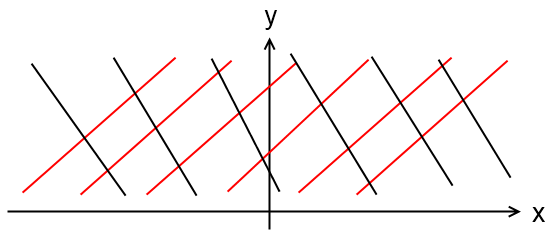
\includegraphics[width=5cm]{Content/01_theory/linksRechts}
\end{minipage}
\subsubsection{Strips/Characteristics}
PDE: $a\partial_x^2u+2b\partial_x\partial_yu+c\partial_y^2u+d\partial_xu+e\partial_yu+fu=g$ Symbol matrix: $ 
	\begin{bmatrix}
		a & b\\
		b & c
	\end{bmatrix}$

Along the curve $t\mapsto(x(t),y(t))$, the initial values / partial derivatives are
$
\left.
\begin{aligned}
u(x(t),y(t))&=u(t)\\
\partial_xu(x(t),y(t))&=p(t)\\
\partial_yu(x(t),y(t))&=q(t)
\end{aligned}
\qquad
\right\}
\label{charanfangs}
$

Characteristics satisfy the ODE:
\[
	a\dot y(t)^2-2b\dot x(t)\dot y(t)+c\dot x(t)^2=0
\]

Characteristic strip additionally satisfies: $a\dot p(t)\dot y(t)-h\dot x(t)\dot y(t)+c\dot x(t)\dot q(t)=0$
